\section*{Part 3: Separation with ICA}

\begin{taskbox}[Part 3: introduction in the lab manual]
In this part we use a technique based on higher-order statistics, Independent Component Analysis (ICA), to separate the maternal, fetal and noise signals. The mixing pattern can be written as ``mixing matrix $\times$ sources $=$ observations'', i.e.\ $\mathbf{X}^{T}=\mathbf{A}\mathbf{Z}^{T}$, where $\mathbf{X}\in\mathbb{R}^{M\times N}$ ($N$ channels, $M$ time samples). The sources are therefore estimated as $\hat{\mathbf{Z}}^{T}=\mathbf{W}\mathbf{X}^{T}$, where $\mathbf{W}$ is the separating matrix and $\mathbf{W}^{-1}$ is an estimate of the mixing matrix $\mathbf{A}$.
\end{taskbox}

\question{3-1}{Computing and saving $\mathbf{W}$, the components and the mixing matrix}

\begin{taskbox}
Apply the ICA technique to the observation matrix $\mathbf{X}^{T}$ using the provided function \texttt{ica}, and obtain and save the matrices $\mathbf{W}$ and $\hat{\mathbf{Z}}$. Then also compute and save the matrix $\mathbf{W}^{-1}$, which is an estimate of the mixing matrix $\mathbf{A}$.
\end{taskbox}

To avoid ambiguity about transposes, the components produced by the code are denoted $\mathbf{S}_{\mathrm{IC}}$ in this report; this corresponds to $\hat{\mathbf{Z}}^{T}$ in the convention of the exercise statement, and the code variable \texttt{Zhat} has size $2560\times3$.
\begin{equation}
\mathbf{S}_{\mathrm{IC}}=\mathbf{W}\mathbf{X}_c^{T},\qquad
\widehat{\mathbf{A}}=\mathbf{W}^{+},\qquad
\mathbf{X}_c^{T}=\widehat{\mathbf{A}}\mathbf{S}_{\mathrm{IC}} .
\label{eq:ica}
\end{equation}
The symbol $+$ denotes the pseudoinverse, which for this full-rank matrix is equivalent to the inverse. In the whitening step, the channel covariance is computed with denominator $M$. Fourth-order cumulants are then estimated and the dominant eigenmatrices are approximately jointly diagonalized.
\begin{align}
\mathbf{W}&\simeq
\begin{bmatrix}
 0.554156 &  0.105982 &  0.407024\\
-0.306577 &  0.512773 & -0.102334\\
-0.062156 & -0.612226 &  0.360719
\end{bmatrix}
\label{eq:W}\\[4pt]
\widehat{\mathbf{A}}&\simeq
\begin{bmatrix}
0.721433 & -1.695245 & -1.294974\\
0.689779 &  1.328220 & -0.401519\\
1.295033 &  1.962201 &  1.867632
\end{bmatrix}
\label{eq:Ahat}
\end{align}
The matrices above are shown rounded to six decimal places; the full versions are in the NPZ file. The order of the columns of $\widehat{\mathbf{A}}$ corresponds to the order of the rows of $\mathbf{S}_{\mathrm{IC}}$. All these matrices were estimated from the observed data only. The reconstruction error with the full matrices is about $7.92\times10^{-16}$.

In the ICA model, a permutation of the sources and a change of scale or sign of one source can be compensated by a corresponding change in its mixing column. In this run the population variance of each component is set to one, so the raw amplitude of the components is a matter of convention.

\question{3-2}{Scatter of the observations and the columns of the ICA mixing matrix}

\begin{taskbox}
Plot the scatter plot of the initial data using \texttt{ch3plot}, and the three sources (components) using \texttt{dv3plot}. Note that \texttt{dv3plot} takes the columns of $\mathbf{W}^{-1}$ as input and can be called several times. Save the resulting figure in \texttt{.fig} format.
\end{taskbox}

\begin{figure}[H]
\centering
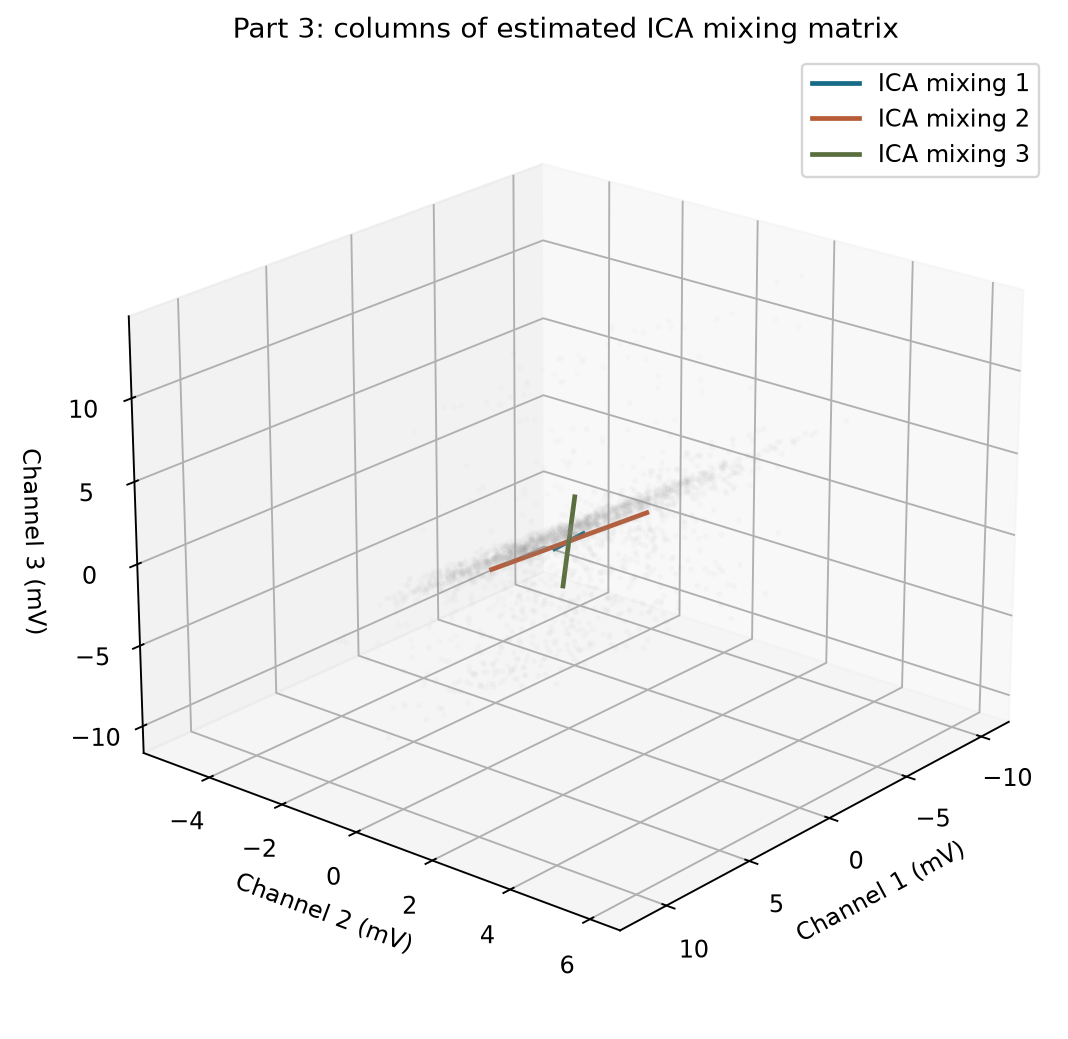
\includegraphics[width=0.66\textwidth]{fig09_ica_mixing_columns_3d.png}
\caption{Directions of the columns of the estimated mixing matrix on the scatter of the observations.}
\label{fig:ica3d}
\end{figure}

Each column of $\widehat{\mathbf{A}}$ shows with what amplitude ratio a separated source appears in the three sensors. Unlike the columns of $\mathbf{V}$, these directions are not necessarily orthogonal in sensor space. This does not contradict the statistical independence of the sources: independence concerns the distribution of the source signals, not necessarily the orthogonality of the mixing columns in sensor coordinates.

To compare directions the vectors must be normalized; comparing the apparent lengths of the lines in this figure and in Figure~\ref{fig:pca3d} is not appropriate, because their display scales differ. The normalized results and the numerical angles are reported in Part~4. The figure is saved in PNG and SVG formats.

\question{3-3}{Plotting the components, selecting the fetus and removing the other contributions}

\begin{taskbox}
Plot the three columns of $\mathbf{W}^{-1}$, or equivalently the three rows of $\hat{\mathbf{Z}}^{T}$. Keep the column of $\mathbf{W}^{-1}$ that, in your opinion, represents the content of the fetal component better than the others, and set the other columns to zero. Using this modified $\mathbf{W}^{-1}$ and the matrix $\hat{\mathbf{Z}}$, return the fetal component to the ECG sensor space.
\end{taskbox}

\begin{figure}[H]
\centering
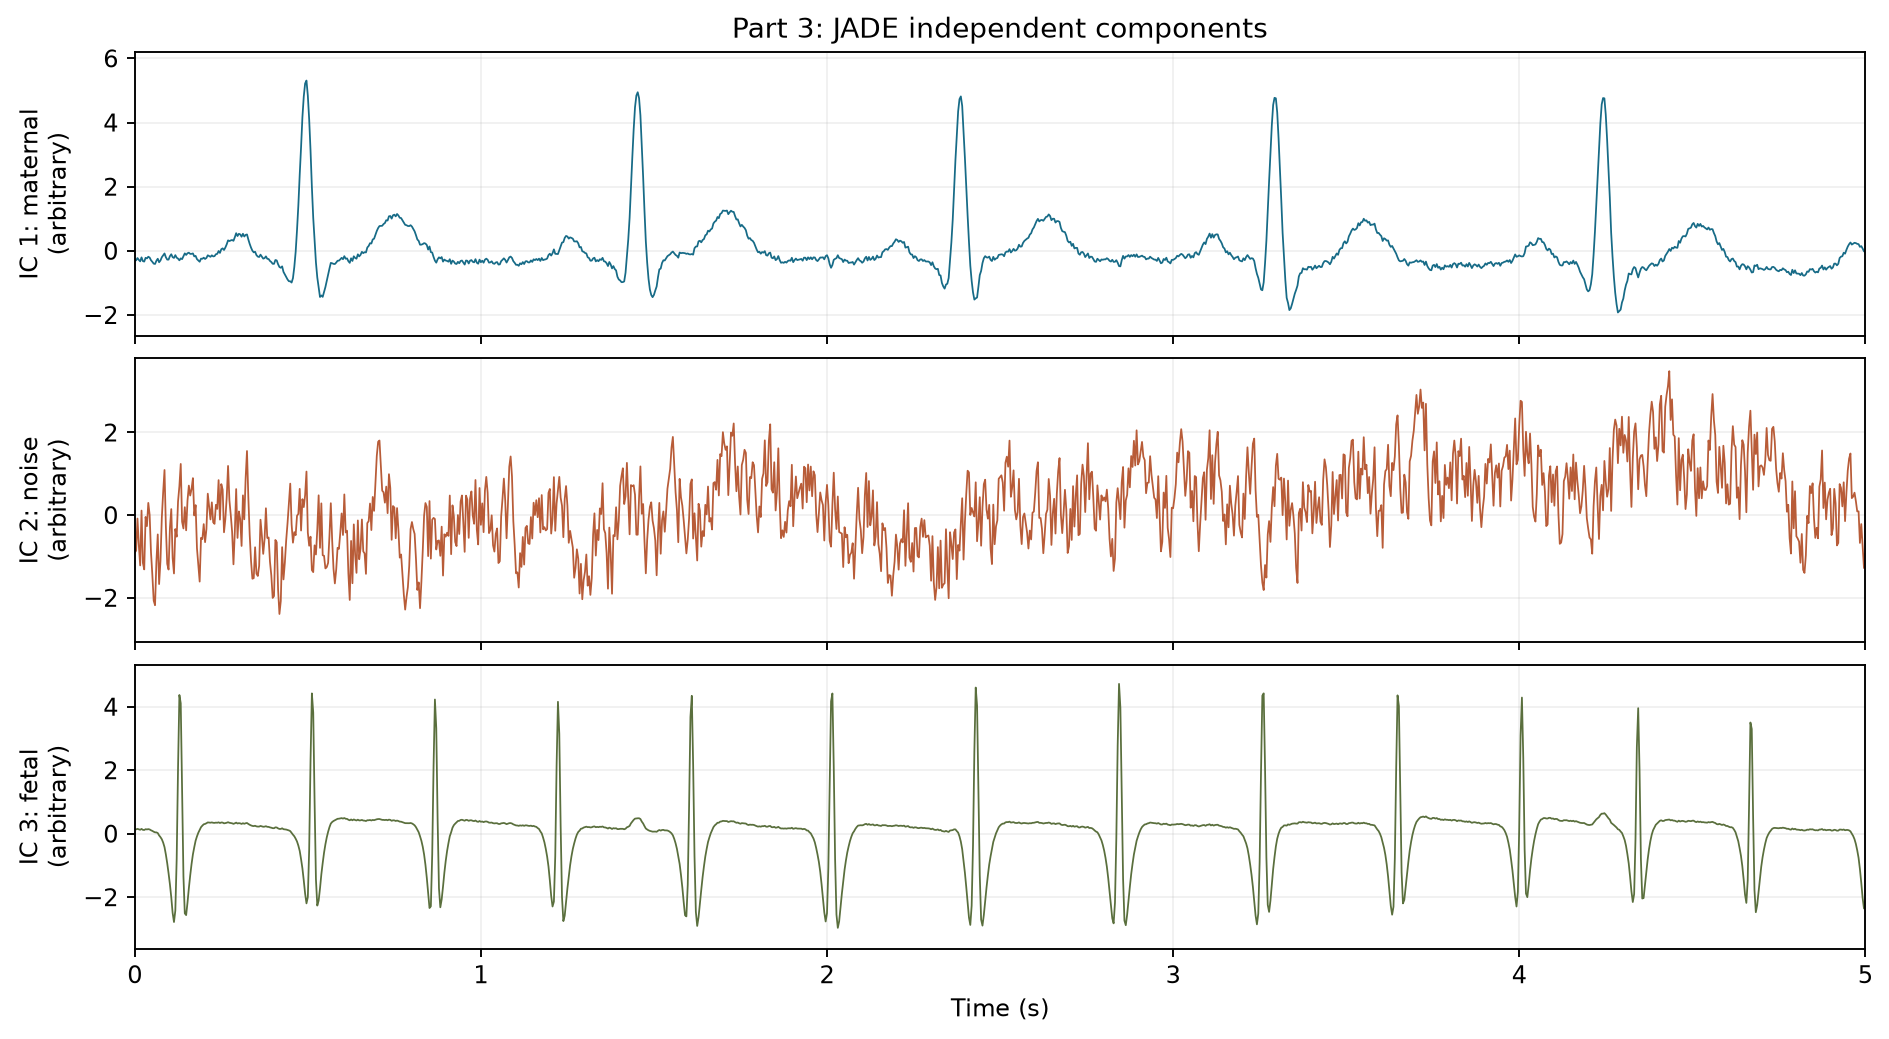
\includegraphics[width=0.95\textwidth]{fig10_ica_components.png}
\caption{The three JADE components in the first five seconds; labels of this run: maternal, noise and fetal.}
\label{fig:icacomp}
\end{figure}

\begin{table}[H]
\centering
\caption{Features of the ICA components; the rate is estimated from the cardiac peaks.}
\begin{tabular}{@{}clrrrr@{}}
\toprule
\textbf{Component} & \textbf{Label} & \textbf{Kurtosis} & \textbf{Peak count} & \textbf{Rate (bpm)} & \textbf{CV(RR)}\\
\midrule
1 & Maternal & 14.560944 & 10 & 62.694 & 0.0757\\
2 & Noise    &  2.845173 &  5 & --     & 0.7017\\
3 & Fetal    &  8.929955 & 26 & 155.152 & 0.0728\\
\bottomrule
\end{tabular}
\end{table}

The first component has slower, regular beats. The second shows irregular oscillations and a kurtosis closer to three. The third has faster, regular beats and was therefore selected as fetal in this run. The rates in the table were obtained from the median interval between peaks found by the same code; a rate extracted from the random peaks of the noise component has no heart-rate interpretation and is therefore not listed.

Keeping only the third column, the fetal contribution in the sensors is reconstructed as
\begin{equation}
\widehat{\mathbf{A}}_f=[\,\mathbf{0}\;\;\mathbf{0}\;\;\hat{\mathbf{a}}_3\,],\qquad
\widehat{\mathbf{X}}_{f,\mathrm{ICA}}=(\widehat{\mathbf{A}}_f\mathbf{S}_{\mathrm{IC}})^{T}.
\label{eq:icafetal}
\end{equation}
In this way the estimated contributions of the mother and of the noise are both set aside. The overall mean of the observations was not added to the fetal contribution, since that mean belongs to the sum of the sources; to reconstruct the whole data set, the stored mean can be added back.

\question{3-4}{Plotting the recovered data and judging the success of ICA}

\begin{taskbox}
Plot and save the data recovered with ICA. In your opinion, was the fetal component recovered successfully?
\end{taskbox}

\begin{figure}[H]
\centering
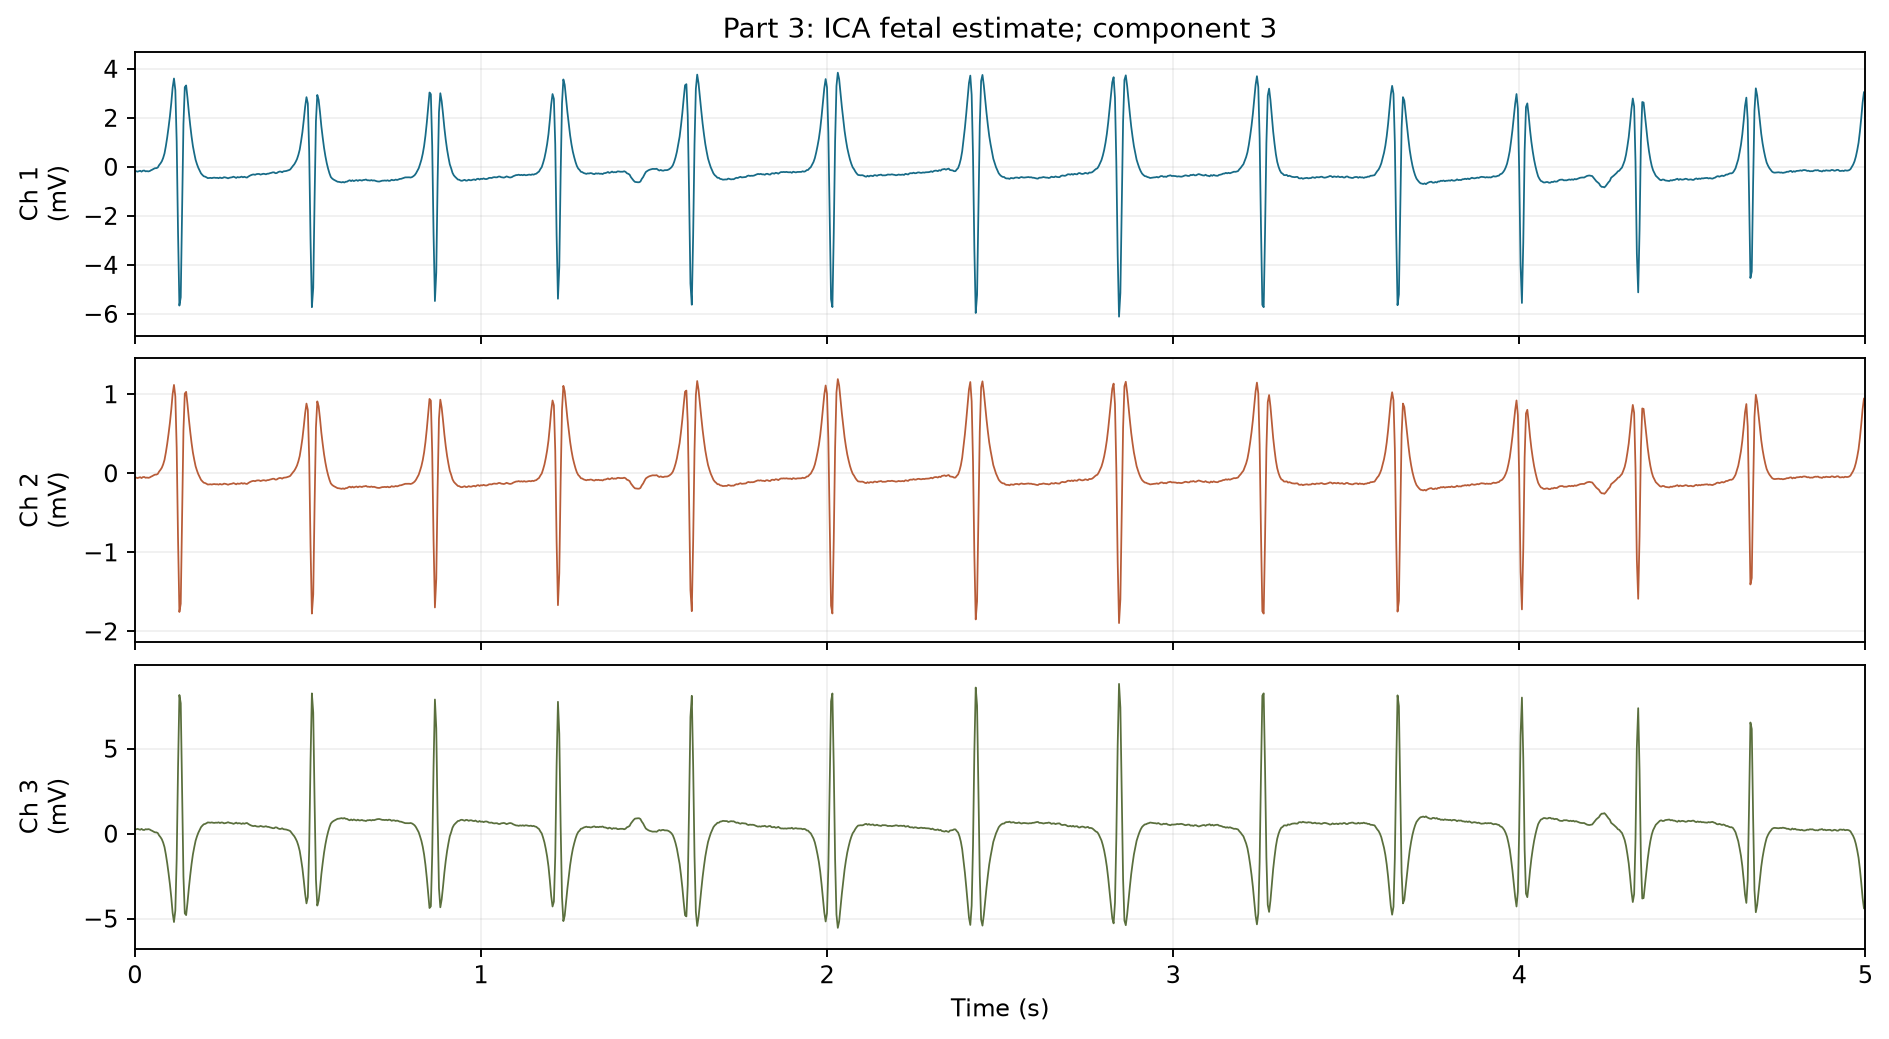
\includegraphics[width=0.95\textwidth]{fig11_ica_fetal_estimate.png}
\caption{Reconstruction of the fetal contribution in the three sensors, keeping ICA component 3.}
\label{fig:icafetal}
\end{figure}

\answer Compared with Figure~\ref{fig:svdfetal}, the fetal beats are more distinct and the interfering oscillations are much less visible. The absolute correlation with the reference is 0.997840, and the normalized error after scale adjustment is 0.065684. Waveform recovery in this simulated record was therefore very successful; the non-zero error shows that the separation is not perfect.

Each of the three rows is the product of one temporal component and three mixing coefficients. Similarity of shape, differences in amplitude and inversion of some channels are therefore natural. A high correlation measures linear similarity; it does not mean ``percent of noise removed'' and is not an independent clinical evaluation.

To clarify the role of the removals, two supplementary outputs are given in the appendix: removing only the noise, which retains both ECG signals, and removing only the mother, which leaves the fetus together with the noise. The output of this question was built by setting aside the contributions of both interfering sources.
